% !TEX root = ../main.tex

\chapter{运动学分析}

\section{引言}

每章的引言起到承接上一章引启下一章的作用。

\ldots\ldots

\section{运动学分析}

考虑三个空间,分别是驱动空间、关节空间以及操作空间。驱动空间包含的是各个绳索长度组成的矩阵,不同时刻绳索长度可能不同。关节空间包含的是机械臂各个关节的关节角组成的矩阵,不同时刻关节角可能不同。操作空间包含的是机械臂末端位姿组成的位姿矩阵,不同时刻位姿可能不同,单个关节三维模型如\figref{fig:bm}所示。

\begin{figure}[ht]
\centering
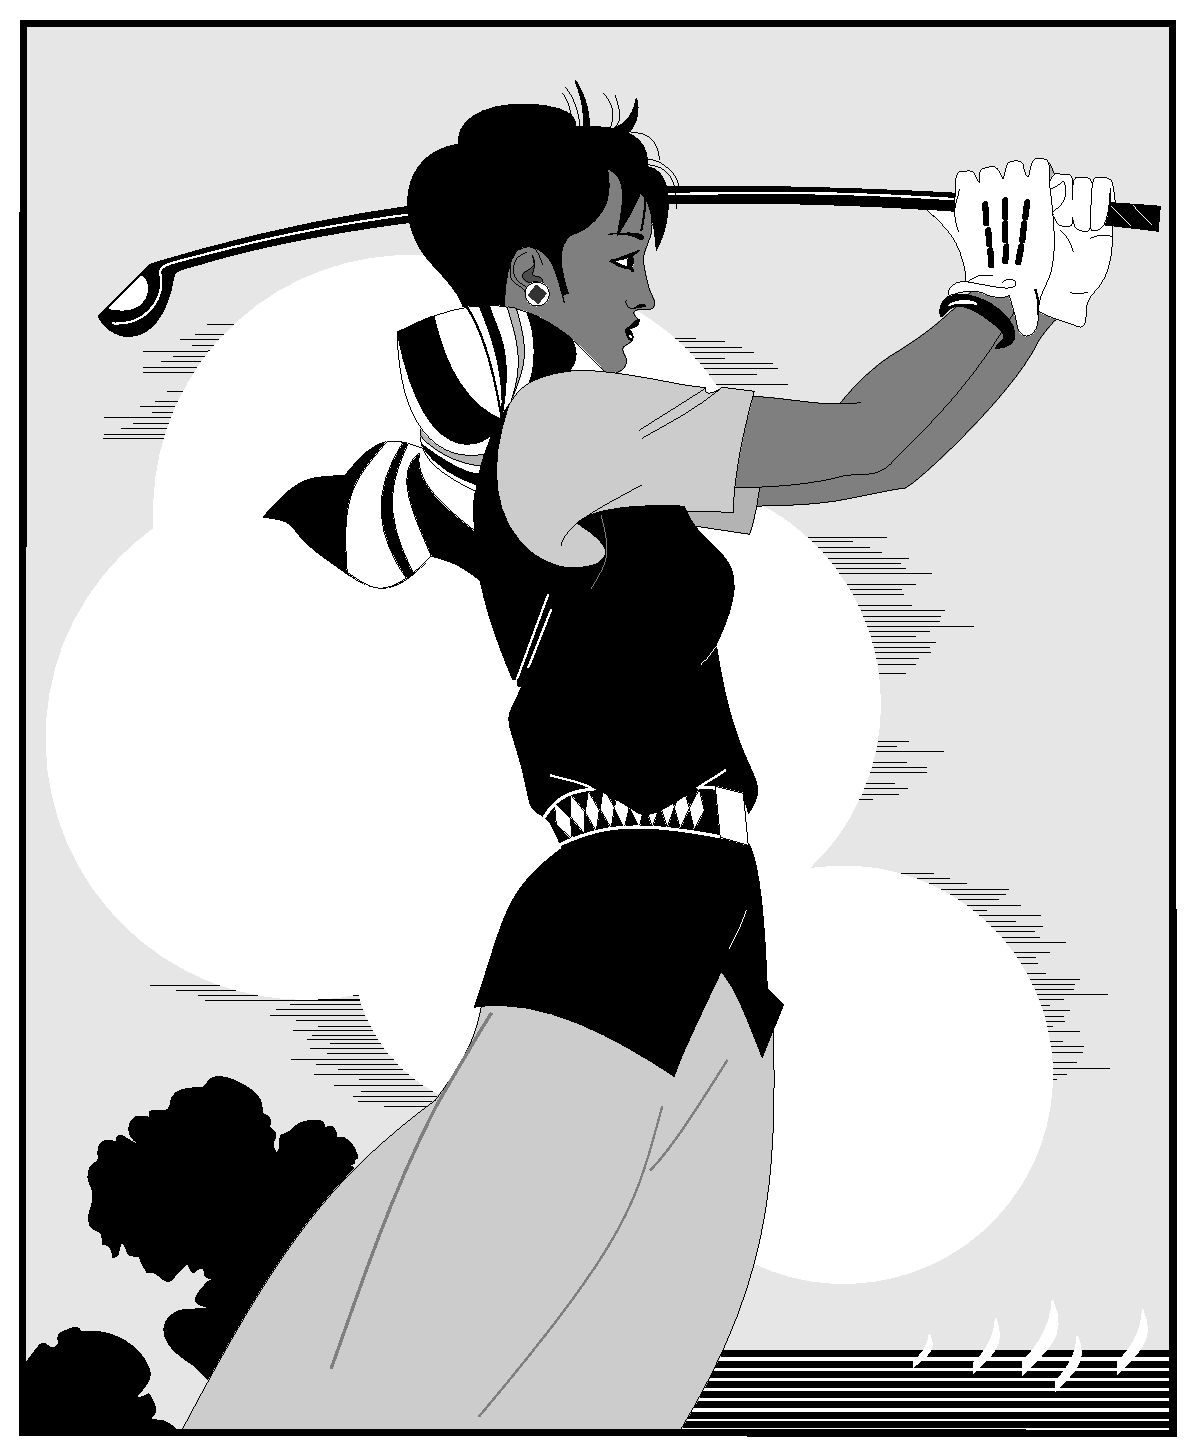
\includegraphics[width = 0.4\textwidth]{golfer}
\caption{打高尔夫球的人}
\label{fig:bm}
\end{figure}

\section{速度级运动学分析}

\subsection{并排图和子图}

位置级运动学的分析过程对速度级运动学的分析有很大帮助。在速度级运动学分析中,绳驱机械臂同样需要考虑三个空间,分别是驱动空间、关节空间以及操作空间。三者之间的关系如\figref{fig:parell1}与\figref{fig:parell2}所示。

\begin{figure}[htbp]
\centering
\begin{minipage}[t]{0.4\textwidth}
\centering
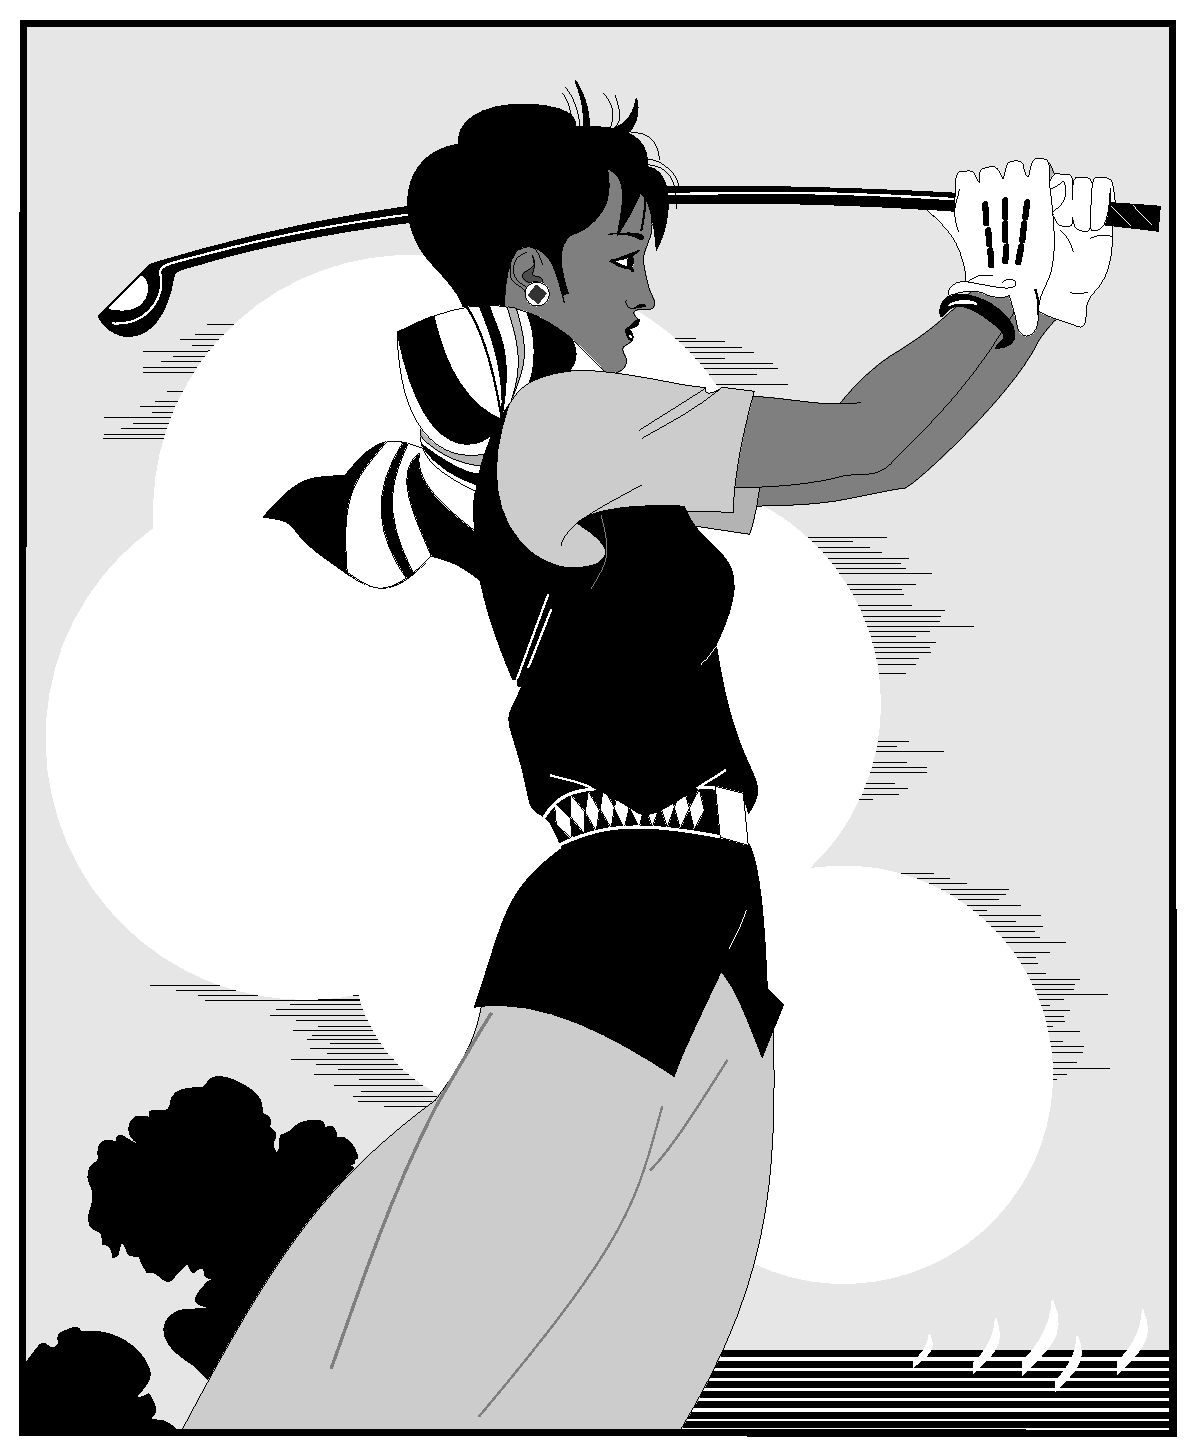
\includegraphics[width=\textwidth,height=\textwidth]{golfer}
\caption{打高尔夫球的人。注意,此图对齐方式是图片底部对齐}
\label{fig:parell1}
\end{minipage}
\centering
\begin{minipage}[t]{0.4\textwidth}
\centering
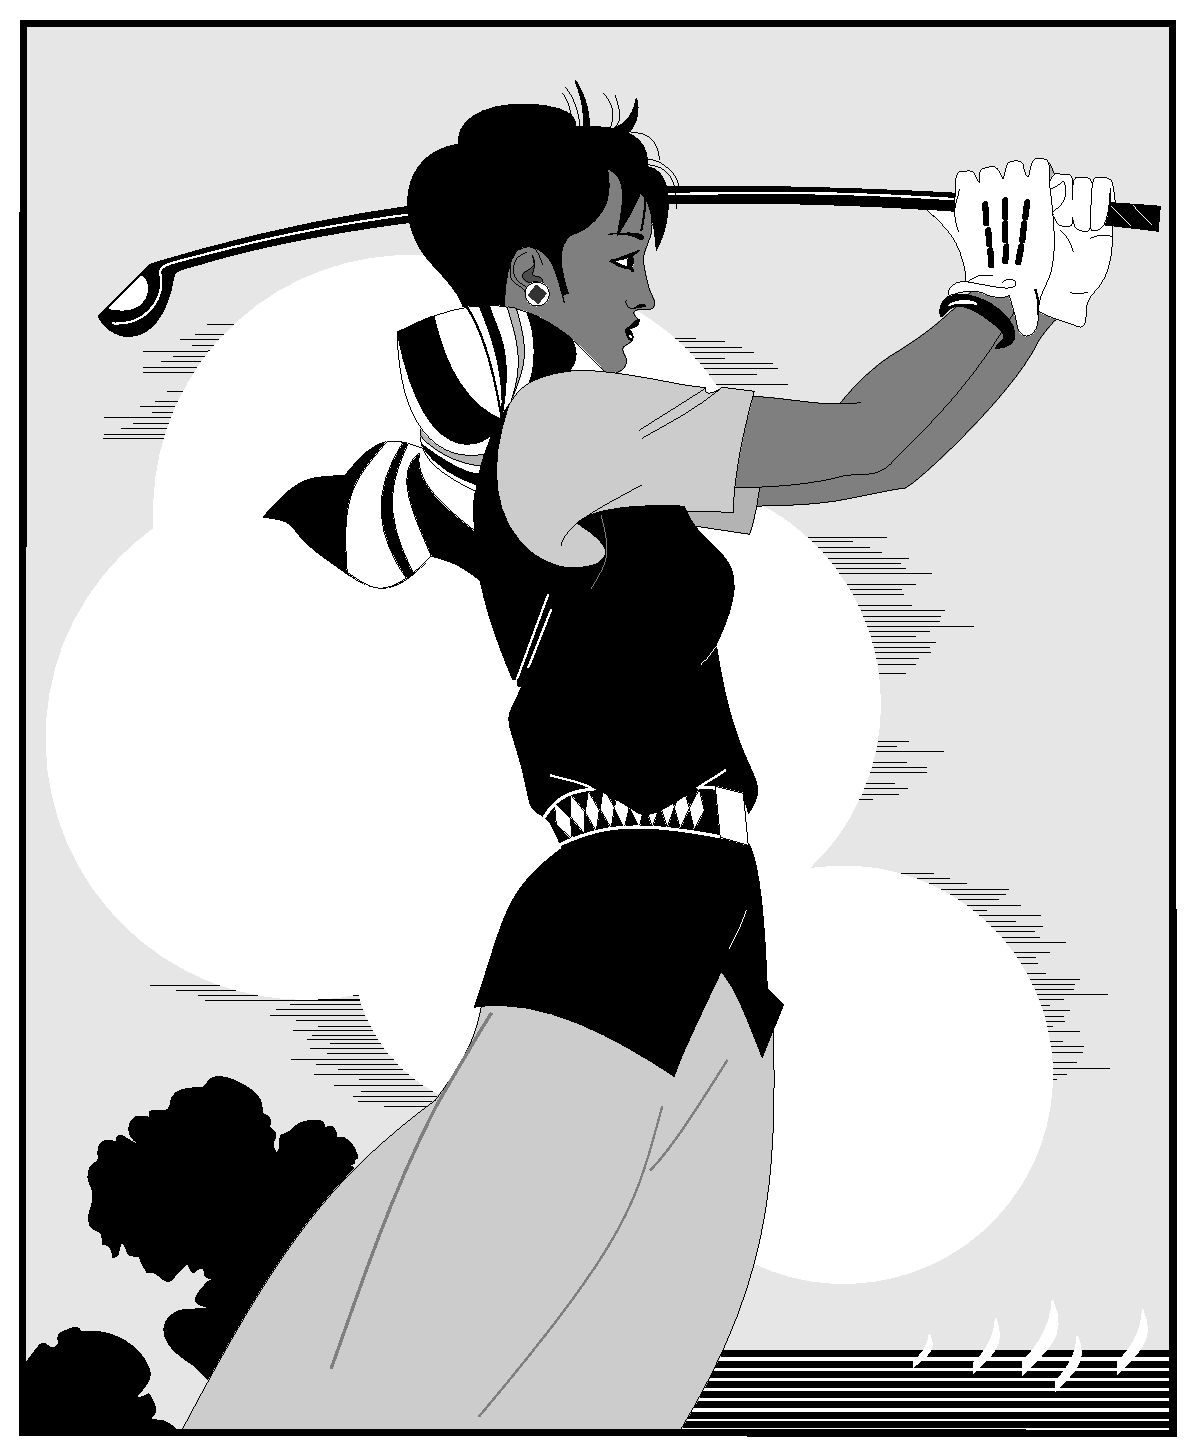
\includegraphics[width=\textwidth]{golfer}
\caption{打高尔夫球的人}
\label{fig:parell2}
\end{minipage}
\end{figure}

\section{本章小结}

总结本章的叙述内容。

\lipsum[1]
